\RequirePackage[hyphens]{url}
\documentclass{article}
\usepackage[a4paper]{geometry}
\usepackage{comment}
\usepackage{graphicx}
\usepackage[ natbib=true, style=numeric,sorting=none,citestyle=numeric-comp]{biblatex}
\addbibresource{ref.bib}
\usepackage{subcaption}
\usepackage{hyperref}
\hypersetup{
    colorlinks,
    citecolor=black,
    filecolor=black,
    linkcolor=black,
    urlcolor=black
}

\title{Machin vs. Machine: Comparing Humans' Ability Against AIs' Ability to Classify Images Into Unsuitable Categories}
\author{Amelie Machin}
\date{2026}

\begin{document}

\maketitle

\begin{abstract}
This paper analyses the differences between how AI and humans react to unexpected situations that force a reliance on past experiences, logical leaps, and guesswork. Specifically, when neural networks, Large Language Models, and humans are tasked with classifying images into classes that poorly or do not at all reflect the contents of the images. It found that\dots
\end{abstract}

\tableofcontents

\section{Introduction}
The human brain is an incredibly complicated example of biological machinery. It can store information and apply it to a variety of situations to efficiently solve problems, complete tasks, understand the world around them, and adapt to change. This allows humans to not only learn from a guide, but from their own mistakes and past experiences. Neural networks are a subcategory of AI that attempts to recreate this behaviour using calculus and matrices. This report aims to discover the differences between how the human brain and neural networks react to unpredictable situations they are ill-equipped to handle, specifically classifying images where none of the categories accurately reflect the image.
\subsection{Neural Networks}
\begin{figure}[hb]
    \centering
    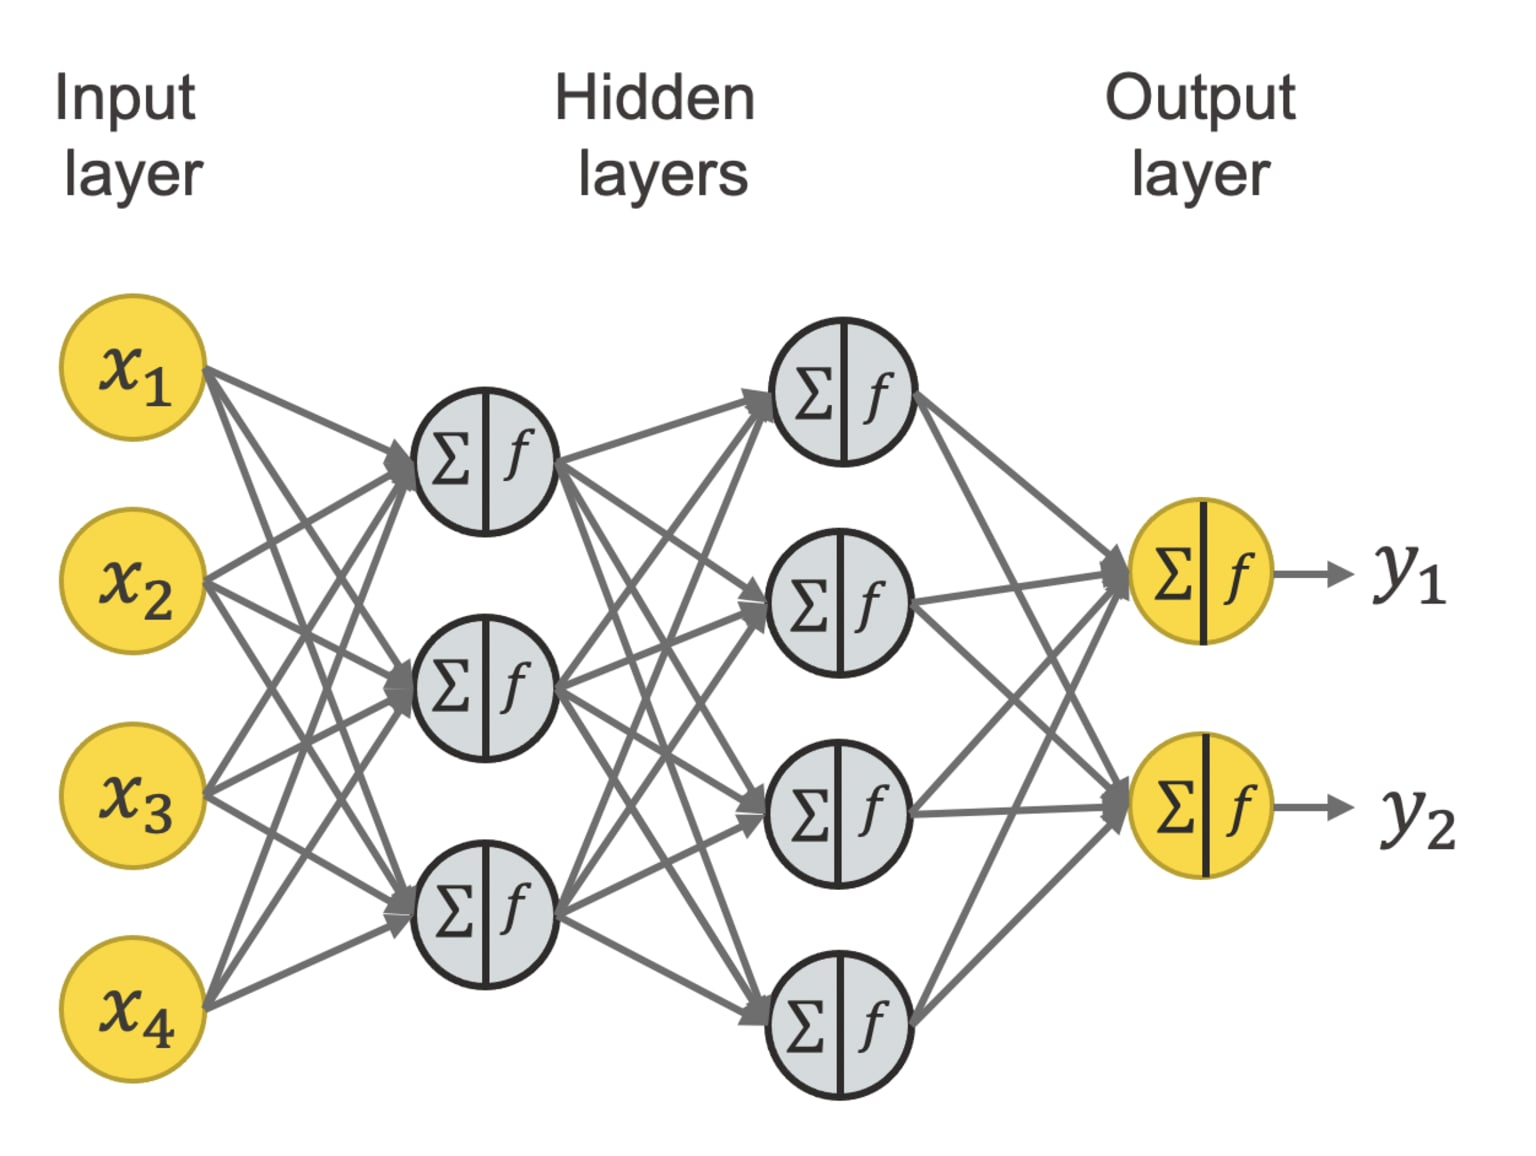
\includegraphics[width=0.75\linewidth]{Images/neuralNet.jpg}
    \caption{A diagram on a neural network with four layers of nodes. $\Sigma$ represents the summation function and $f$ represents the activation function. Taken from \url{https://www.knime.com/blog/a-friendly-introduction-to-deep-neural-networks}}
    \label{fig:netimage}
\end{figure}
\noindent Neural networks are a branch of AI that mimic the structure of neurons in the human brain. They consist of layers of nodes that can receive multiple inputs, process, and output a real number [Fig. \ref{fig:netimage}]. As the machine learns, its outputs get closer and closer to a predicted output.  Each node always performs the same process with the sum of its inputs (the summation function), but the influence that node has on the final output changes as the machine learns. This change in output is from changing the weight of each node (the process of applying the weight to the output is called the activation function). The way the network decides the weight of a node is based on its learning paradigm. The paradigm this research focuses on is supervised learning, but other paradigms such as unsupervised or reinforcement learning exist \cite{lampropoulos2015machine}.


\subsection{Image Recognition}
Image recognition is an application of machine learning and neural networks where images are classified into categories based on the contents of the image.
\begin{figure}[ht]
    \centering
    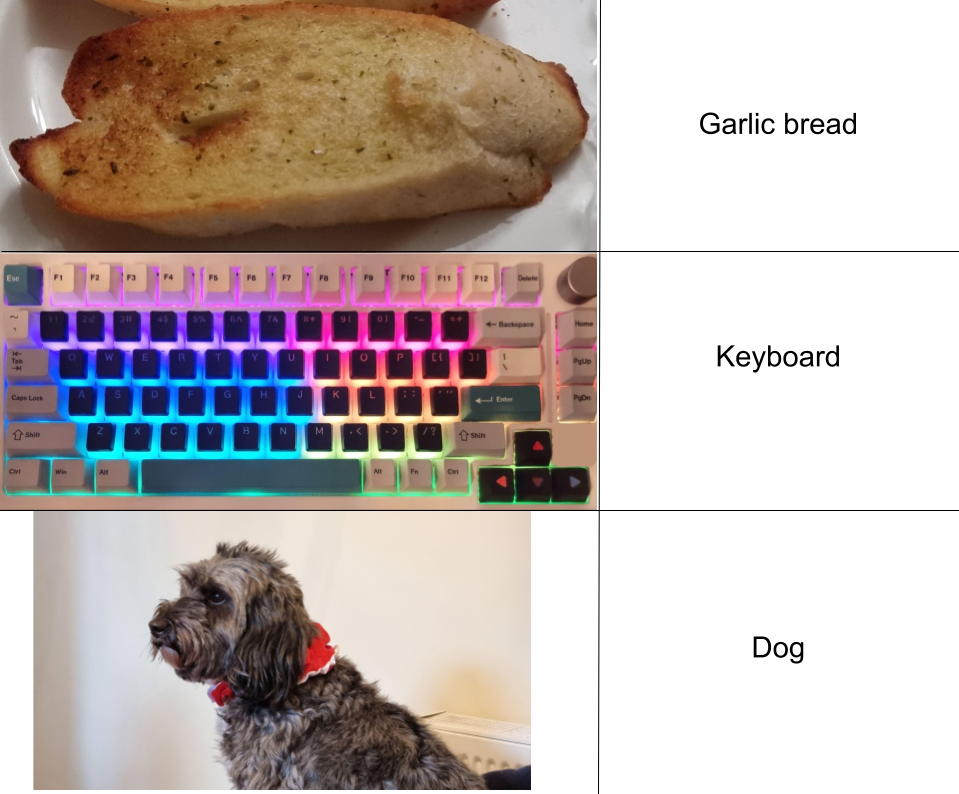
\includegraphics[width=0.9\linewidth]{Images/supervisedImages.png}
    \caption{An example of images from a supervised dataset, with images on the left and labels for the images on the right.}
    \label{fig:supimages}
\end{figure}

Supervised learning is a common paradigm for image recognition \cite{krizhevsky2012imagenet}. This is because it trains the neural network by generalising connections between characteristics found in the data and the label the data has been manually given by humans \ref{fig:CIFARImages}[Fig. \ref{fig:supimages}], and changing the weights of the nodes accordingly. This suits image recognition as, during training, the neural network can generalise the links between characteristics it finds within the image and the given labels, and use these generalisations to make predictions.


\subsection{Large Language Models}
Large Language Models (LLMs) are a subsection of Artificial Intelligence that have been trained on vast amounts of data in order to process and generate natural language \cite{bommasani2022opportunitiesrisksfoundationmodels}. Common examples include OpenAI's ChatGPT \cite{ChatGPT}, Google's Gemini \cite{Gemini}, and Microsoft's Copilot \cite{Copilot}.


\subsection{Zero-Shot Inference}
Zero-shot inference is where a neural network is given a task it has not been explicitly trained to do \cite{mehta2025generalizationtheoryzeroshotprediction}. In image classification, this means forcing the network to classify images into categories it has not been specifically trained to identify.

As LLMs are trained on vast amounts of data, it is unlikely that the network is completely unfamiliar with the categories it is given. Here, "zero-shot" refers to providing the LLM with a prompt that contains no examples for what fits into each category, nor does it include descriptions of features to look out for. It is usually only given the category names, and the images to classify.


\section{Literature Review}
\textbf{Generalisation in humans and deep neural networks \cite{geirhos2018generalisation}} --
Geirhos et al. aimed to compare the success rate of humans against deep neural networks when tasked with recognising distorted images. These distortions mainly focussed on changing the colours or amount of noise in the image. They found that humans were mostly more accurate on average at identifying distorted images than the networks for non-colour related distortions, where the networks always had a higher average accuracy. They also found that human participants’ responses were distributed almost entirely equally, whereas the networks showed increasing biases towards certain categories as the distortions got stronger.

I have included 2 distortions that were not used in this study: kaleidoscope and liquefy. These distortions, unlike the distortions used by Geirhos et al., change the shape of the object in the image. 


\section{Methodology}

\subsection{The Classes}
The classes form the foundation for how every area of this research is structured, so choosing the right set was essential. These classes needed to be from a dataset that I could train a neural network off of, easily recognisable for humans with little to no explanation, and small in number so that people do not get overwhelmed when choosing a class for an image, while still having enough classes for patterns to form in the results (around 5-10 classes seems ideal).

\begin{figure}[ht]
    \centering
    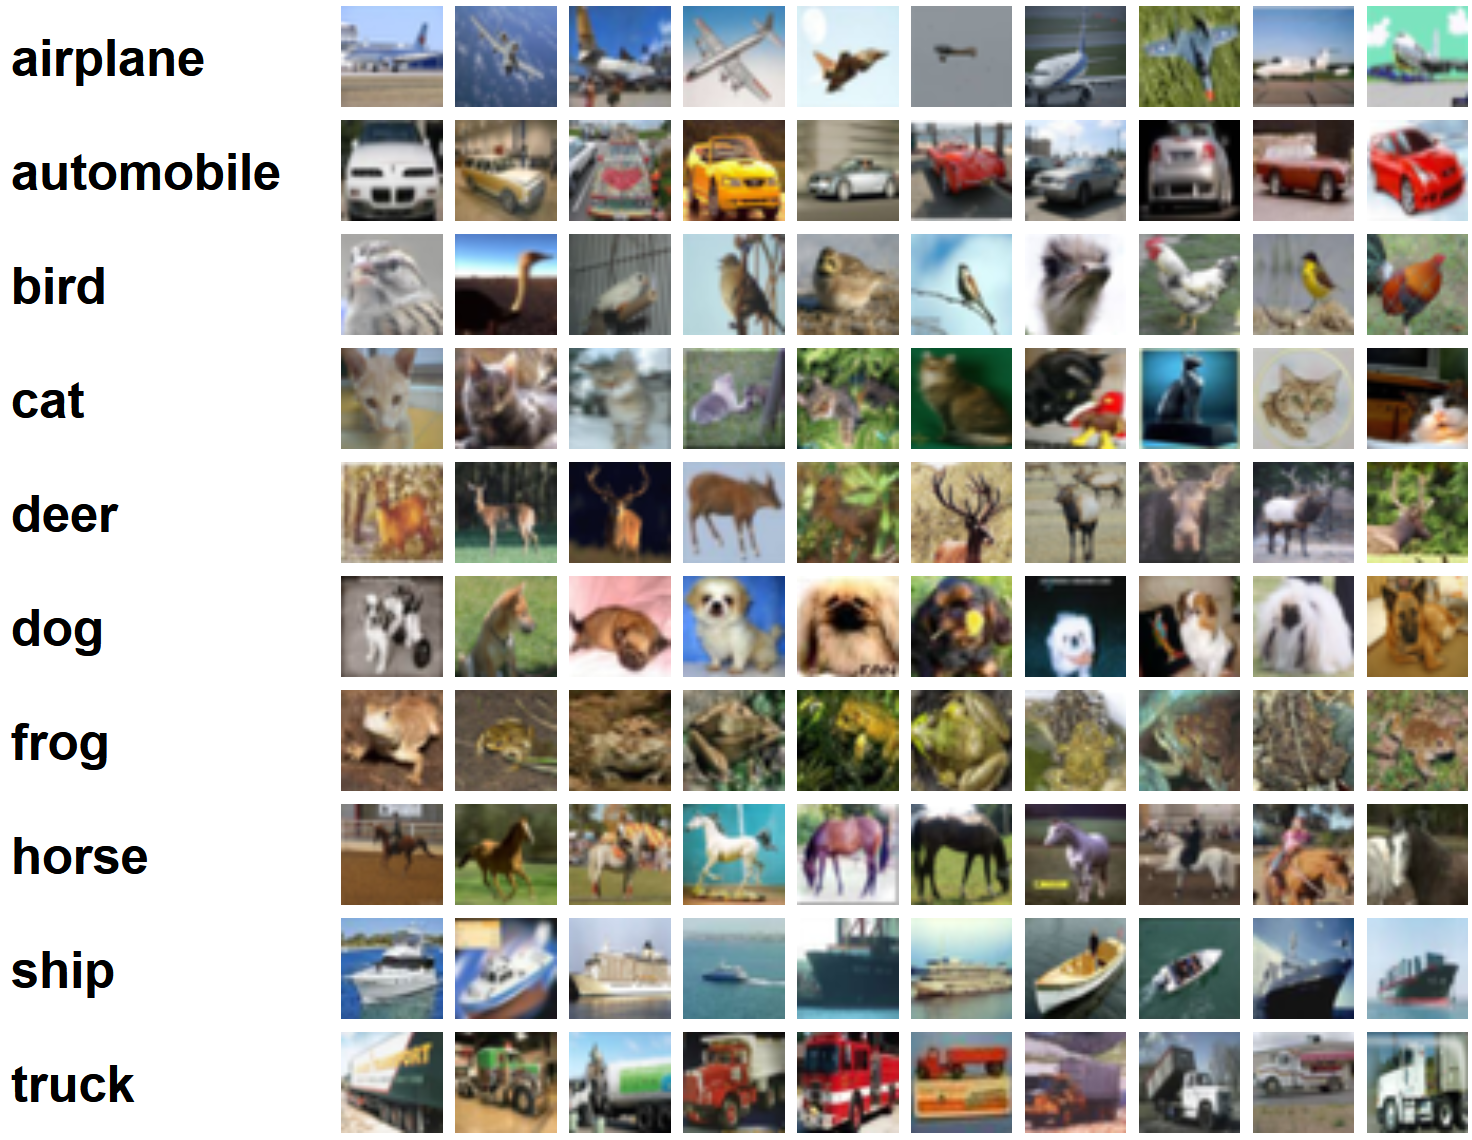
\includegraphics[width=0.75\linewidth]{Images/CIFARImages.png}
    \caption{Example images for each class in the CIFAR-10 dataset. Taken from: \url{https://www.cs.toronto.edu/~kriz/cifar.html}}
    \label{fig:CIFARImages}
\end{figure}

Some of the most popular datasets include ImageNet, CIFAR-10, CIFAR-100, CALTECH-101, and CALTECH-256 \cite{bestDatasets}. Out of thee datasets, the only one with a low enough number of classes is CIFAR-10, one of the most popular datasets for research into image classification \cite{krizhevsky2009learning}. It has 10 classes of common objects and 60000 images, so perfectly fits my criteria [Fig. \ref{fig:CIFARImages}].


\subsection{The Test Data}
\begin{figure}[ht]
    \centering
    \begin{subfigure}[t]{0.16\textwidth}
        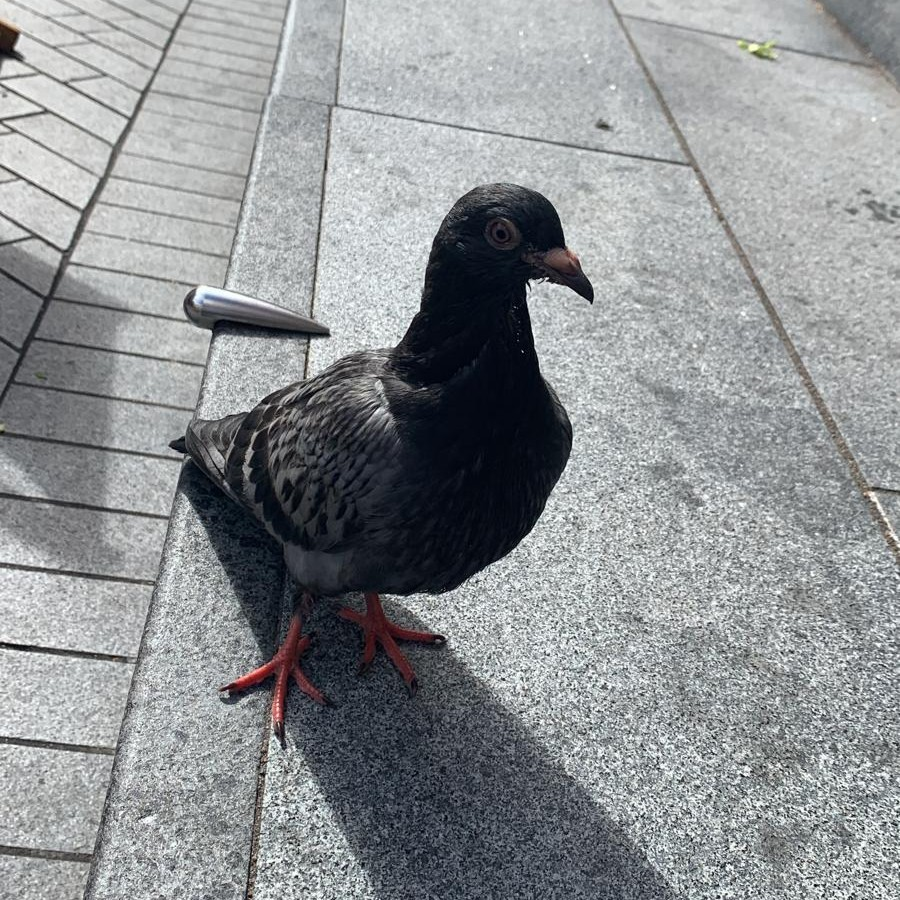
\includegraphics[width=0.95\linewidth]{../Images/pigeon.jpg} 
        \caption{Image 1: A pigeon}
        \label{fig:pigeon}
    \end{subfigure}
    \begin{subfigure}[t]{0.2\textwidth}
        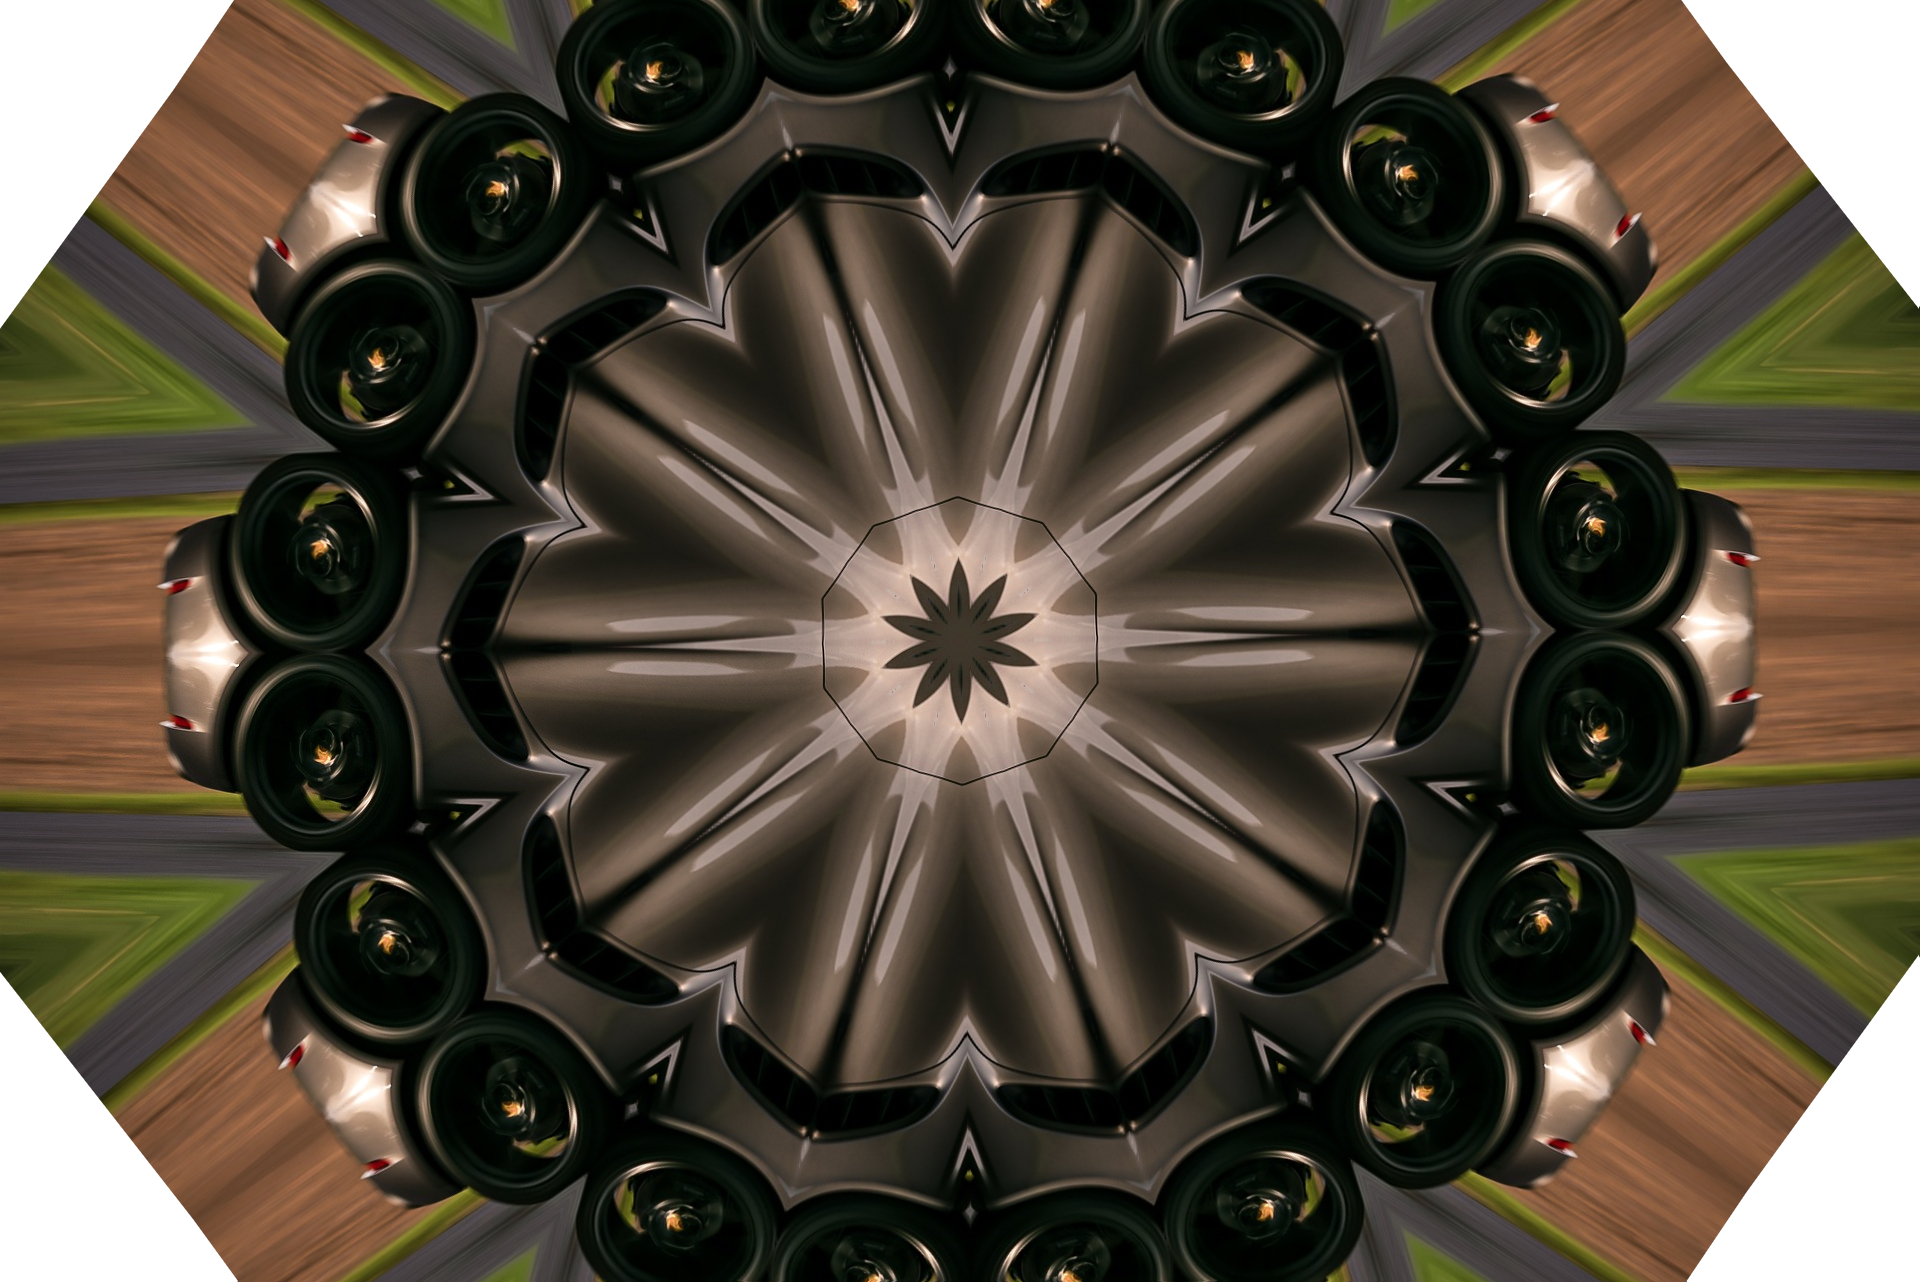
\includegraphics[width=0.95\linewidth]{../Images/automobileKale.jpg}
        \caption{Image 2: A car after a kaleidoscope effect has been applied}
        \label{fig:automobileKale}
    \end{subfigure}
    \begin{subfigure}[t]{0.2\textwidth}
        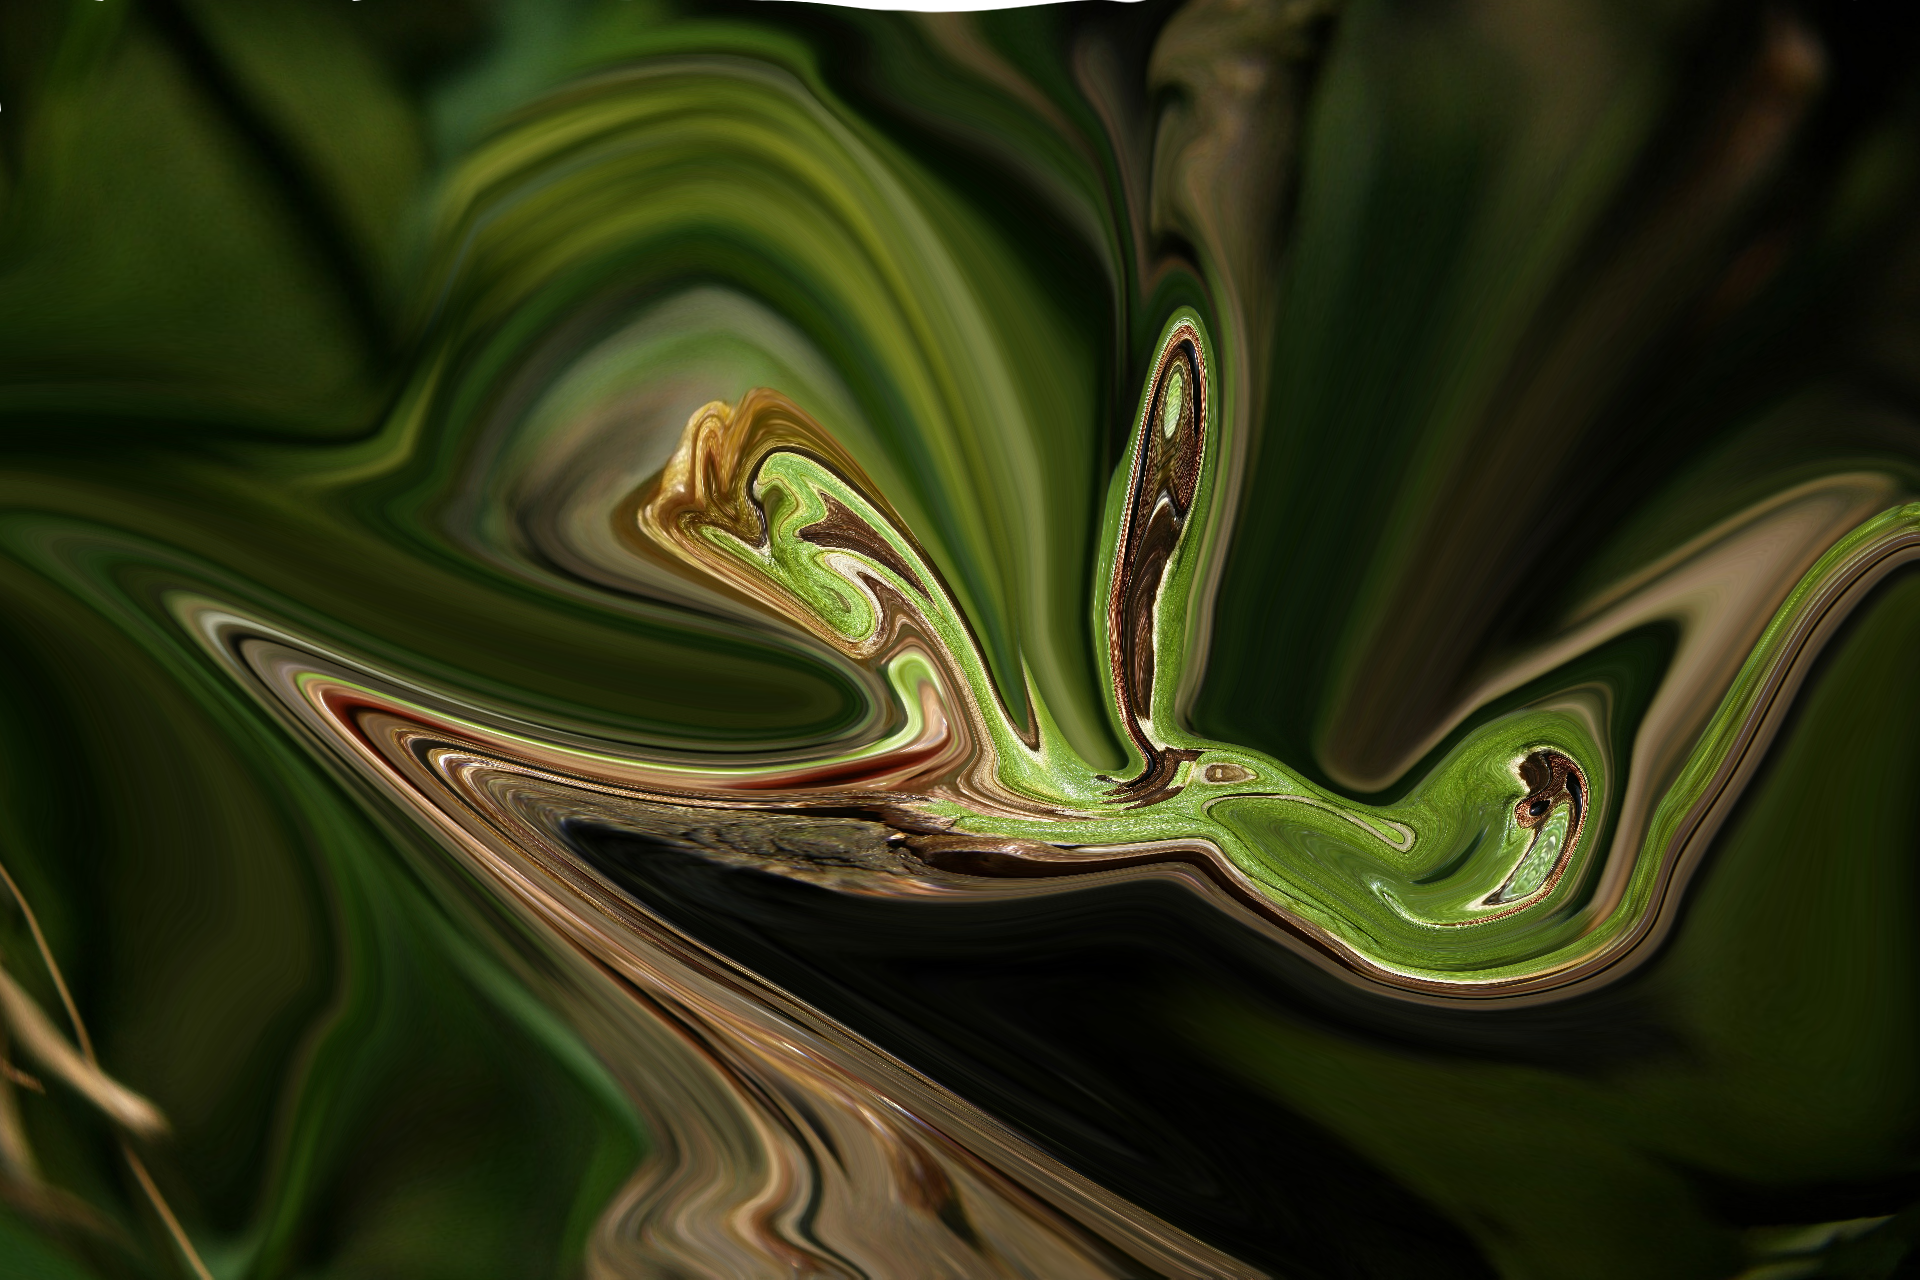
\includegraphics[width=0.95\linewidth]{../Images/treeFrogWarp.png} 
        \caption{Image 3: A frog after a liquefy effect has been applied}
        \label{fig:treeFrogWarp}
    \end{subfigure}
    \begin{subfigure}[t]{0.2\textwidth}
        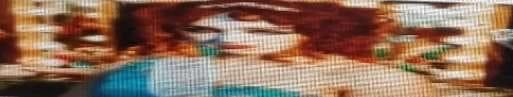
\includegraphics[width=0.95\linewidth]{../Images/Chappell.jpg} 
        \caption{Image 4: The singer Chappell Roan after a squish effect has been applied}
        \label{fig:Chappell}
    \end{subfigure}
    \begin{subfigure}[t]{0.19\textwidth}
        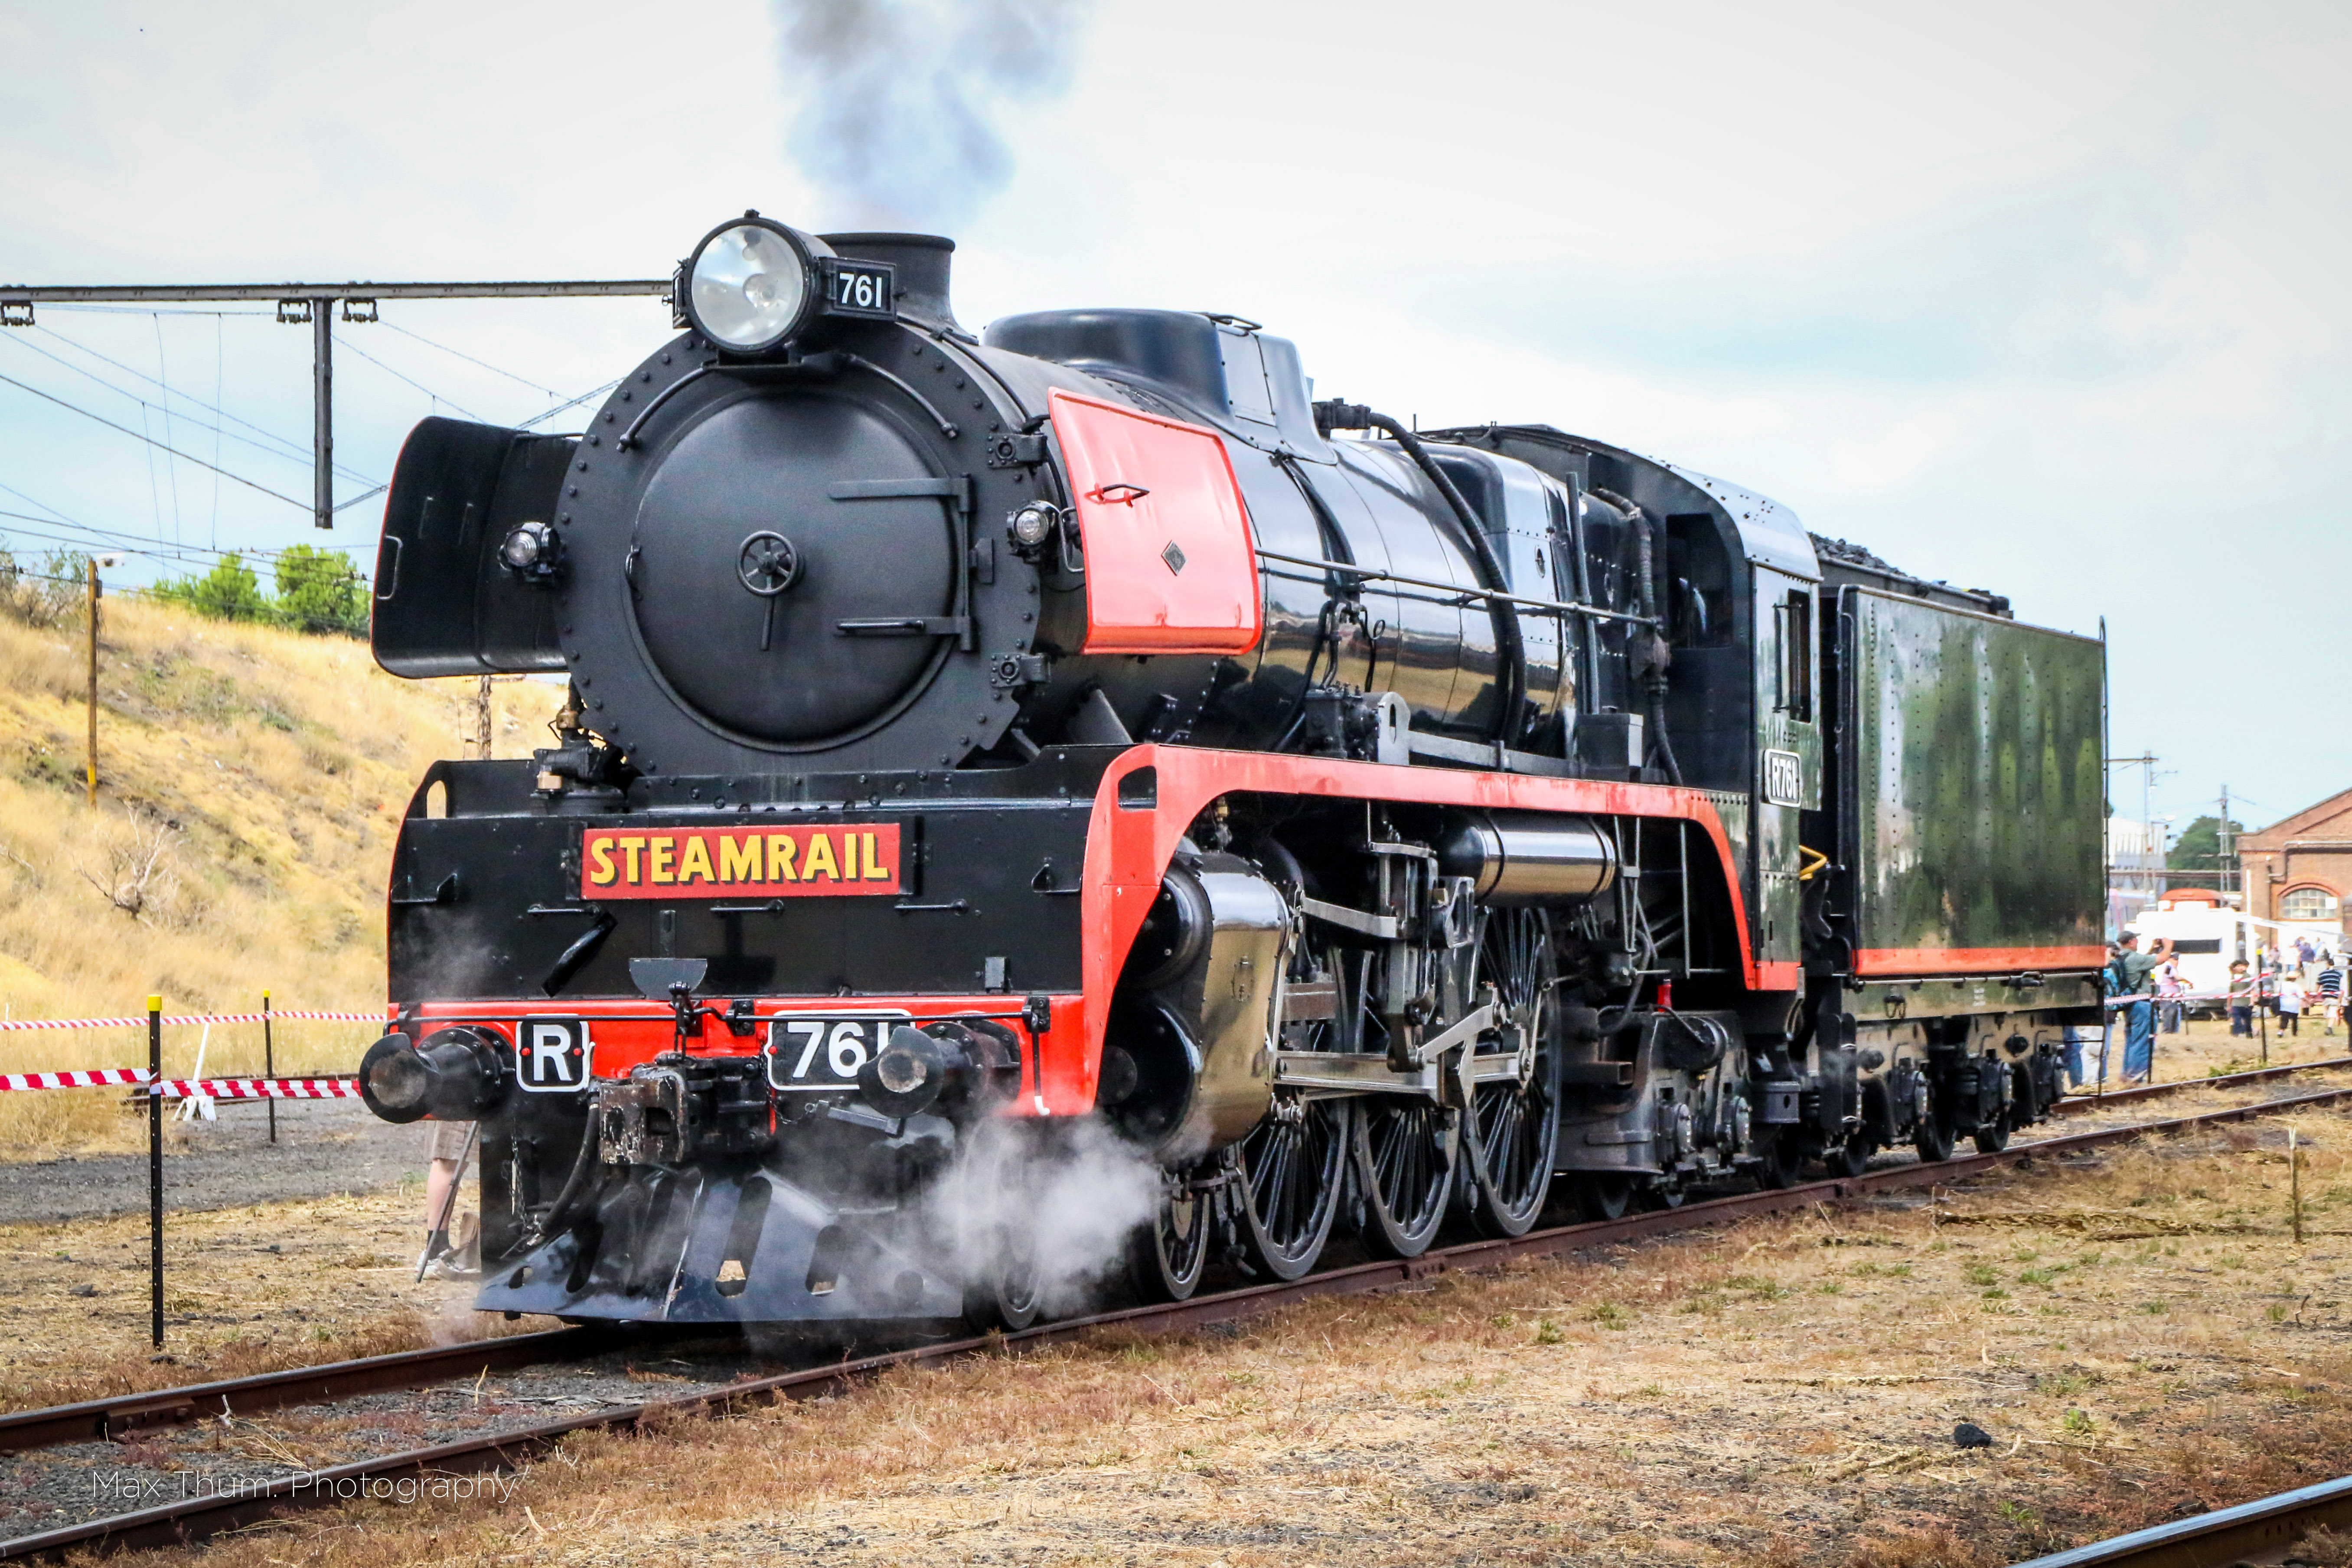
\includegraphics[width=0.95\linewidth]{../Images/train.jpg} 
        \caption{Image 5: A train}
        \label{fig:train}
    \end{subfigure}

    \begin{subfigure}[t]{0.2\textwidth}
        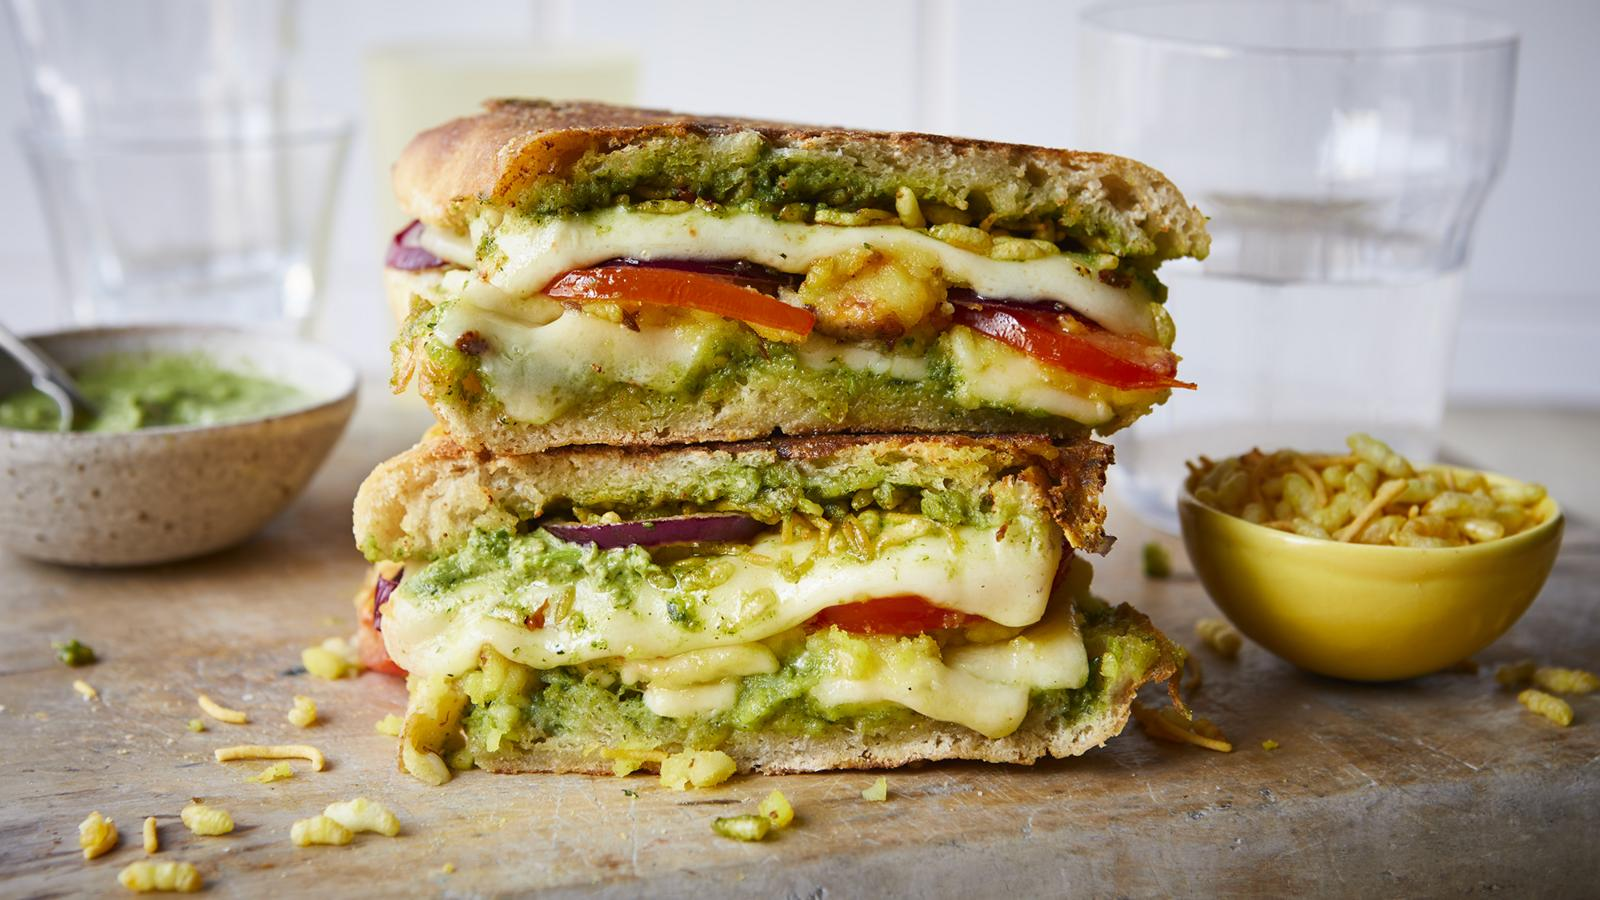
\includegraphics[width=0.95\linewidth]{../Images/sandwich.jpg} 
        \caption{Image 6: A sandwich}
        \label{fig:sandwich}
    \end{subfigure}
    \begin{subfigure}[t]{0.2\textwidth}
        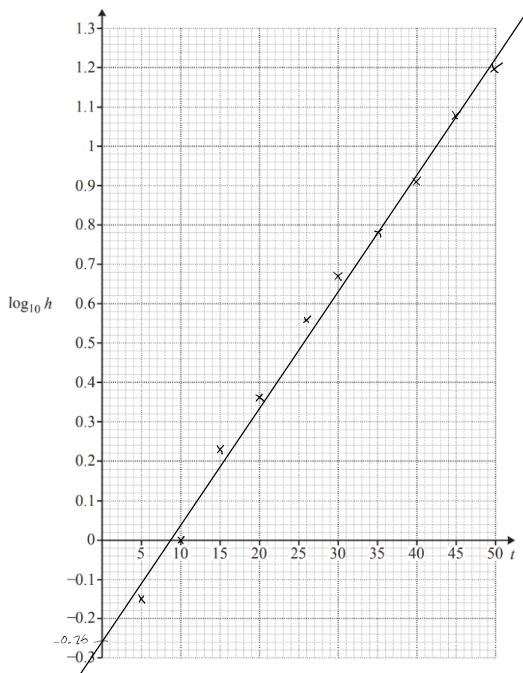
\includegraphics[width=0.95\linewidth]{../Images/Graph.png} 
        \caption{Image 7: A graph}
        \label{fig:Graph}
    \end{subfigure}
    \begin{subfigure}[t]{0.18\textwidth}
        
\includegraphics[width=0.95\linewidth]{../Images/drinkCan.jpg} 
        \caption{Image 8: A can of Coca-Cola}
        \label{fig:drinkCan}
    \end{subfigure}
    \begin{subfigure}[t]{0.17\textwidth}
        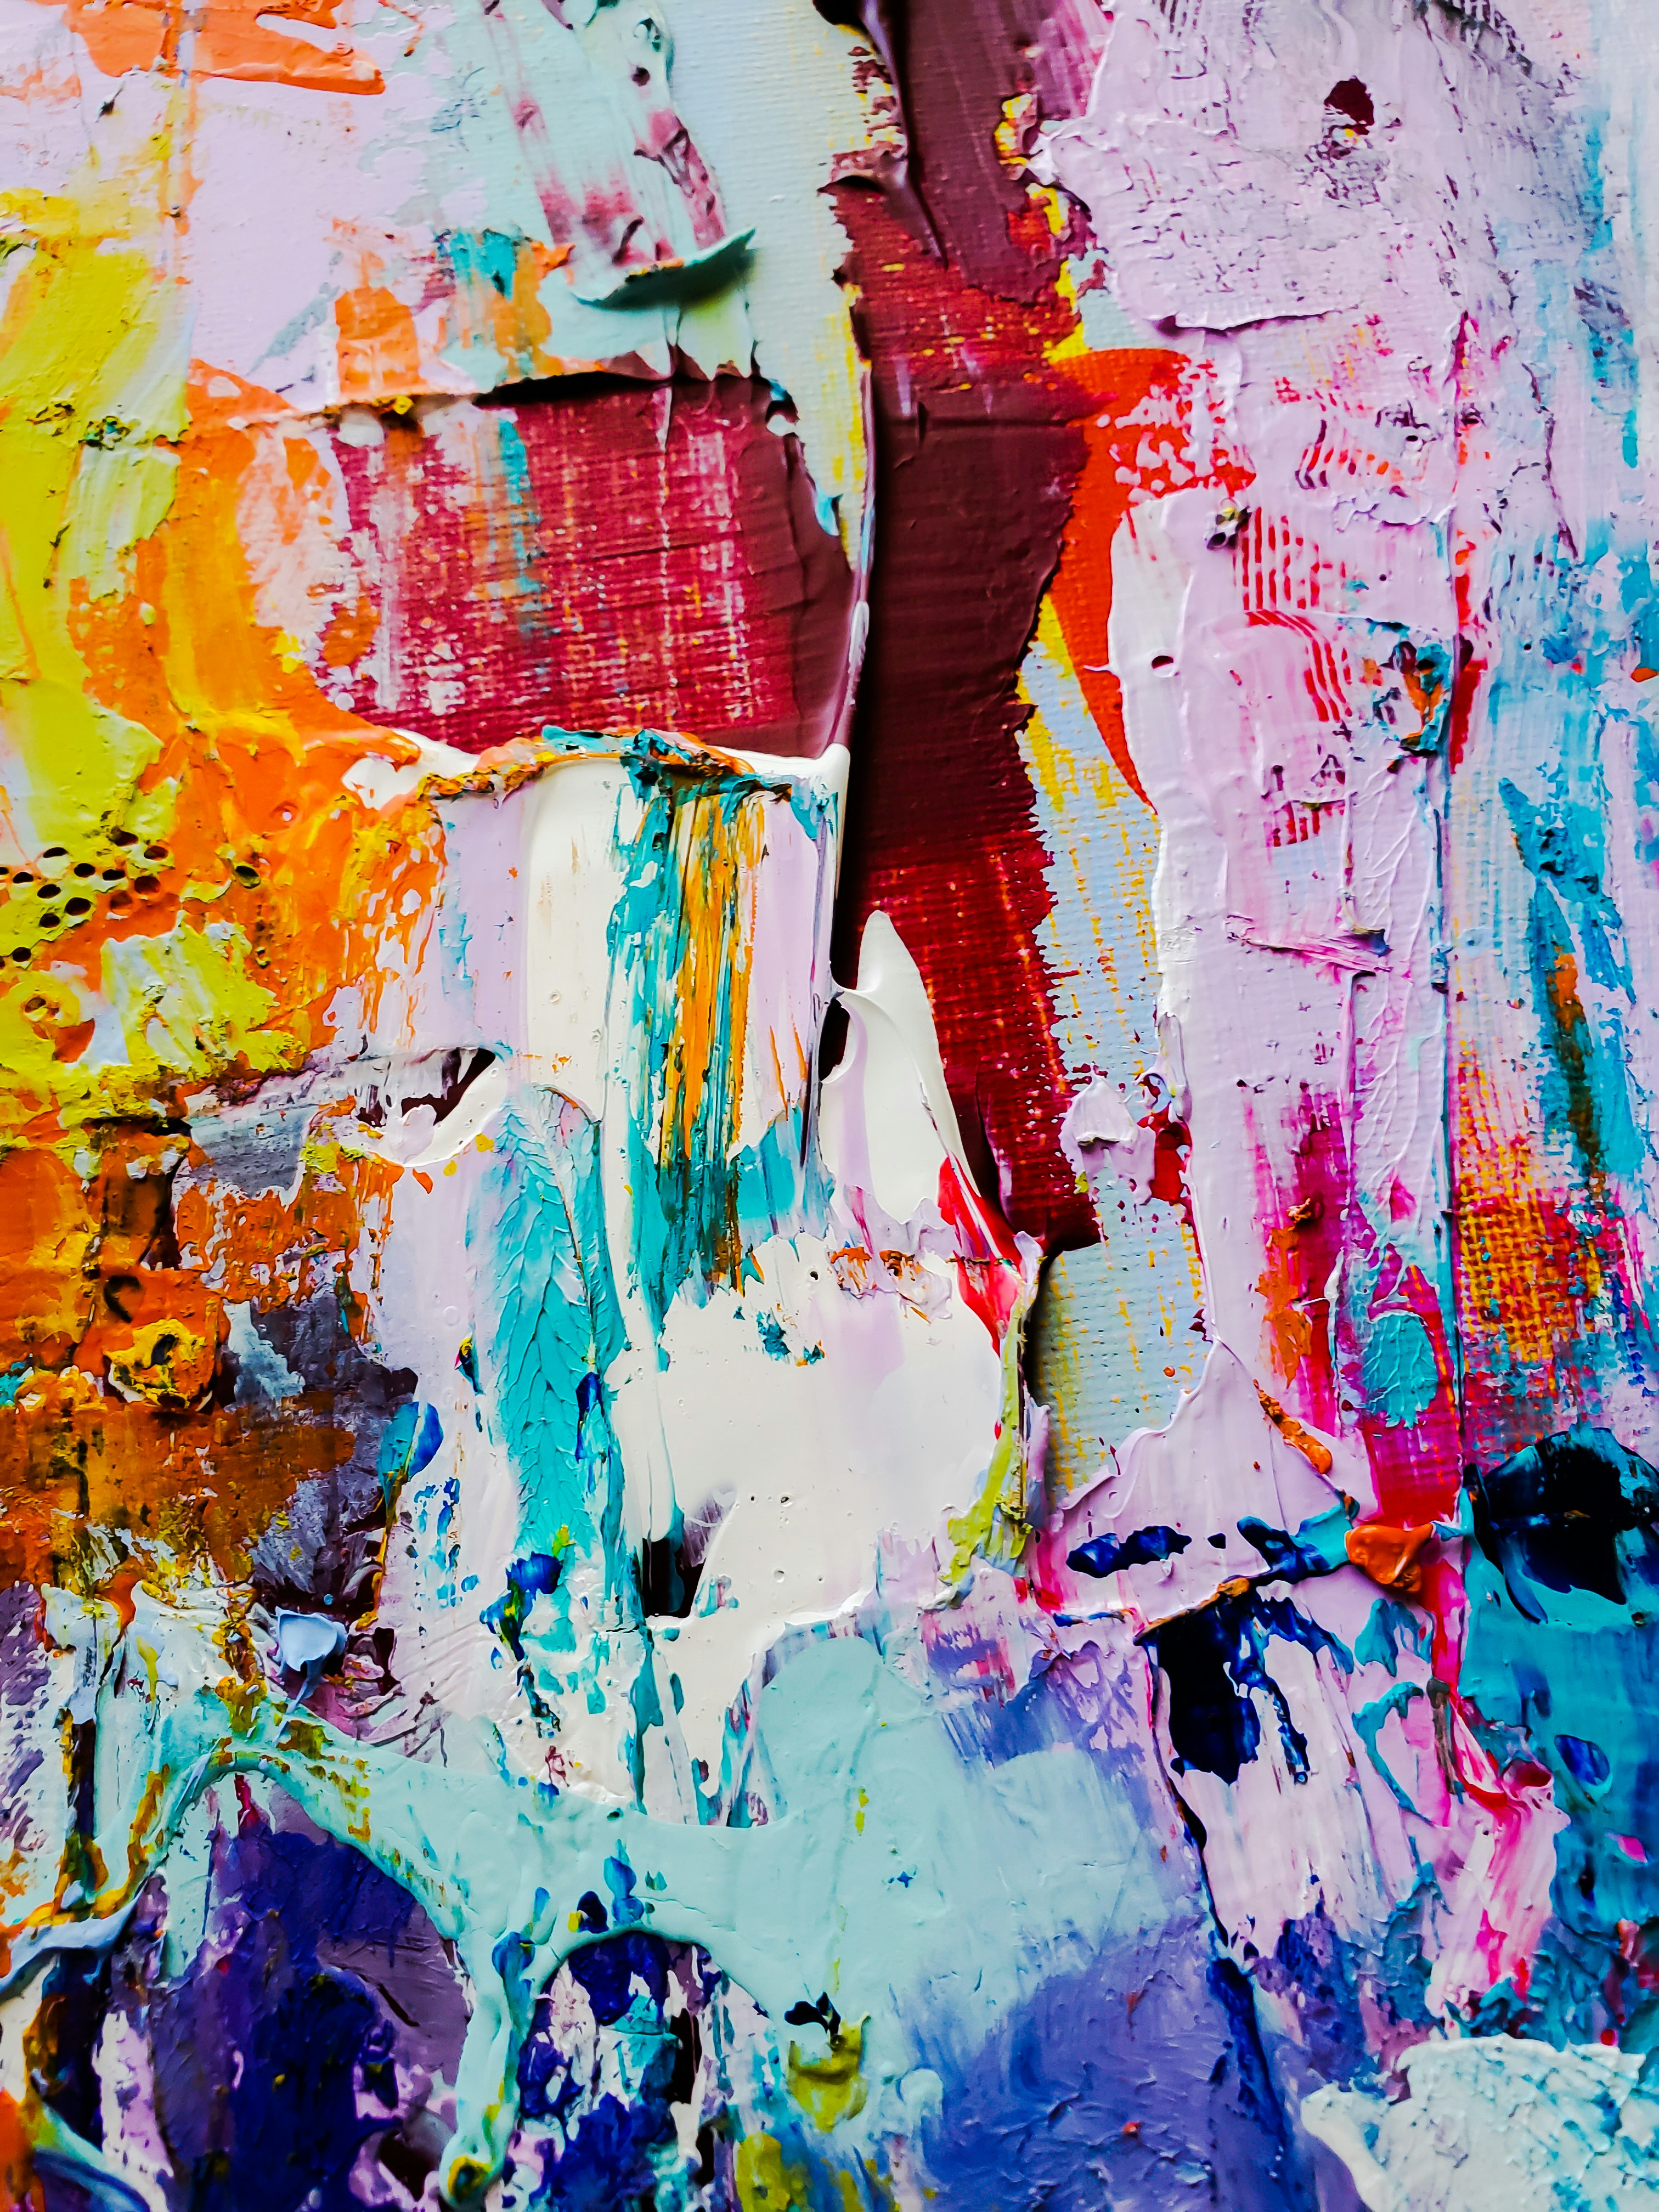
\includegraphics[width=0.95\linewidth]{../Images/abstract.jpg} 
        \caption{Image 9: A painting}
        \label{fig:abstract}
    \end{subfigure}
    \begin{subfigure}[t]{0.2\textwidth}
        \includegraphics[width=0.95\linewidth]{../Images/weirdShape.jpeg} 
        \caption{Image 10: A Roman dodecahedron}
        \label{fig:weirdShape}
    \end{subfigure}
    \caption{The images used for testing. Sources in section \ref{Sources}}
    \label{fig:testImages}
\end{figure}
I needed to create a set of images that would make every class appear to be an unsuitable description of the image, but in different ways. For example, I used an image of an abstract painting [Fig. \ref{fig:abstract}] as it has no logical links to any of the CIFAR-10 classes. However, I also used an image of a train [Fig. \ref{fig:train}] as it could be linked to the "automobile" or the "truck" classes as they are all vehicles, but neither category accurately reflects the image.

I added the pigeon image [Fig. \ref{fig:pigeon}] as a control to test the reliability of the gathered data, and the automobile [Fig. \ref{fig:automobileKale}] and frog [Fig. \ref{fig:treeFrogWarp}] images as I was inspired by research into the effect of distorted images in "Generalisation in humans and deep neural networks" \cite{geirhos2018generalisation}, and wanted to extend their research by looking into shape-warping distortions.

Every image used can be seen in [Fig. \ref{fig:testImages}]


\subsection{Creating a Neural Network}
\begin{figure}[ht]
    \centering
    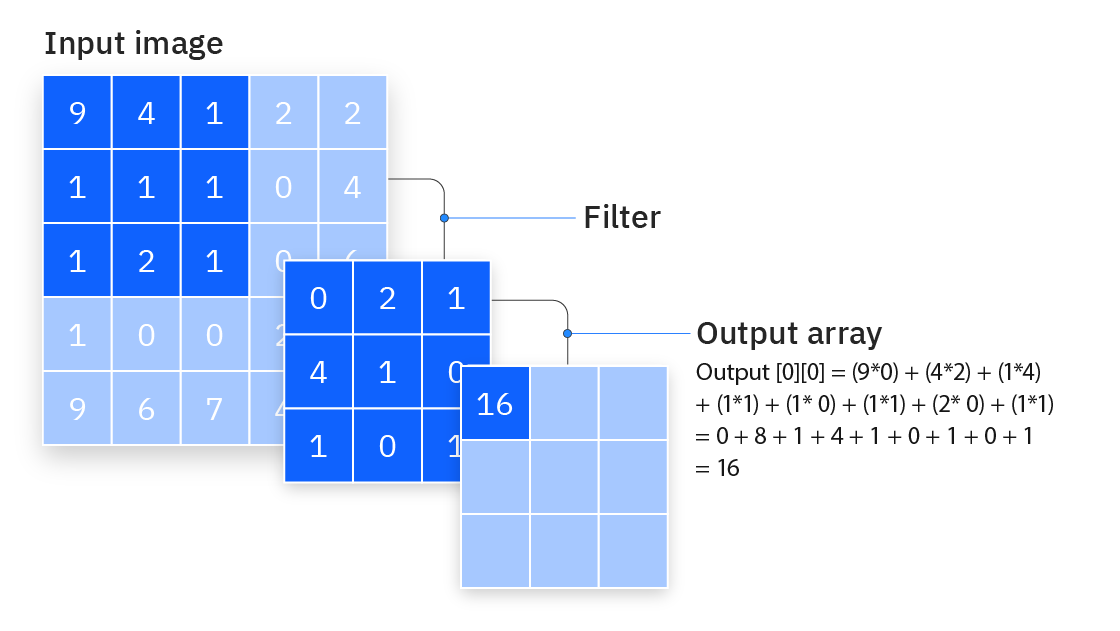
\includegraphics[width=1\linewidth]{Images/convolution.png}
    \caption{The process of convolution. The input image represents the pixels in the image, or the output array of previous iterations. The output array is another term for a feature map. Source: \url{https://www.ibm.com/think/topics/convolutional-neural-networks}}
    \label{fig:convolution}
\end{figure}
I created a Convolutional Neural Network (CNN) in Python using TensorFlow's Keras library and trained it on CIFAR-10's training dataset \cite{krizhevsky2009learning}. When an image is inputted into it, it outputs the most likely class, and a confidence score as a percentage. The layout is as follows:
\begin{itemize}
    \item Convolution layer [Fig. \ref{fig:convolution}] -- The image is split into groups of pixels, 3x3 in size, stored as matrices. A dot product is calculated between each matrix of pixels and a filter. A filter is a matrix that tests for the likelihood of a certain feature being present in an image. These filters change as the CNN learns. These dot products then come together to form a feature map, which shows where the feature the filter was testing for is in the image.
    \item ReLU -- An activation function that executes immediately after convolution. For each value in the feature map, negative values become 0 and positive values remain constant. It allows the CNN to learn non-linear as well as linear relationships between feature and classification. 
    \item Max pooling layer -- Reduces dimensions on the feature map by converting a group of 2x2 pixels into one pixel that takes the greatest value within the group.
    \item Each of the above is repeated twice more, for three of each.
    \item Fully-connected layer -- Uses a softmax function to give a probability of how likely each feature corresponds to each category.
\end{itemize}

I have taken two precautions to prevent overfitting (where the CNN is too accurate with the training data, such that it is very inaccurate with the unseen testing data). One is data augmentation, which is where small, random adjustments are applied to the images before training \cite{shorten2019survey}. The other is dropout (at a rate of 0.5), which is where nodes are randomly disabled to prevent the CNN from focussing to closely on certain features and enable the CNN to make more general and robust links between feature and classification \cite{srivastava2014dropout}.


I used Python because it is the language I am most experienced with, and it is the most popular language for machine learning, thanks to its machine learning libraries such as TensorFlow, Scikit-learn, PyTorch, and Keras \cite{overflow2022libraries,newhorizons2023pythonML}.


I used Keras because of its extensive documentation that guided me through every step \cite{kerasDocs}. Its syntax was also the most intuitive for me out of the most popular libraries, so I was able to get started with coding faster.


I chose to create a Convolutional Neural Network because the convolutional layer, that is exclusive to CNNs, lends itself well to image recognition as it mimics the human process of looking for recognisable features \cite{rawat2017CNN}.

\subsection{Retraining Publicly Available Neural Networks}
I have retrained the InceptionV3 \cite{szegedy2014goingdeeperconvolutions} and ConvNext \cite{liu2022convnet2020s} neural networks using transfer learning. Both neural networks were originally trained on ImageNet \cite{ImageNet}, an image dataset with over 14 million images and 100,000 categories.

Transfer learning is where only the final layer of the neural network is changed from its initial training, to after it has been retrained. This means that most of the nodes, weights, and functions stay the same, but the final output is changed. Int his case, this means that instead being able to classify images into one of 100,00 categories, it can only classify into the 10 CIFAR-10 categories with very little training needing to be done.

I chose these neural networks because they were the only models in Keras' library that supported 32x32 images, which CIFAR-10 images are.


\subsection{Using Zero-Shot Inference with Large Language Models}
I provided 4 web-based Large Language Models (ChatGPT, Gemini, Copilot, and Claude) and 1 Python-based Vision-Language Model (CLIP) with the following prompt and attached the images alongside it.
\begin{quote}
    You will be given 10 images, and you must classify these images into a category based on the contents of the image. These categories are: airplane, automobile, bird, cat, deer, dog, frog, horse, ship, truck. For some images, none of these categories may seem suitable, but you must select from one of these categories, and give a reason behind your choice. Please also rate how well your chosen category reflects the contents of the image, between 1 and 10 inclusive. The images are attached.
\end{quote}

\subsection{Survey}
I created a survey using Google Forms and sent it out via friends of friends and online survey swapping websites. The respondents were asked the same three questions for each of the 10 images, with the images being in the order shown above [Fig. \ref{fig:testImages}]. The questions and multiple-choice options were as follows.
\begin{enumerate}
    \item What category would you select for this image? \\ Options: Airplane; Automobile; Bird; Cat; Deer; Dog; Frog; Horse; Ship; Truck.
    \item Why did you pick that category? \\ Options: It fit the image the best; Random choice; Just chose the first/last/other option; Drawn to that category; Don't know; Other (Custom responses).
    \item How well does the category you chose fit the image, in your opinion? \\ Options: Integers 1 through 10.
\end{enumerate}

\subsection{Modelling the Results}
I used the programming language R to process and model the results of my neural network, the LLMs, and the survey separately.

I omitted all data that failed to identify the pigeon as a bird. 

I plotted the categories chosen for each image as\dots
I plotted the confidence ratings for each image as\dots
I also plotted overall confidence ratings for the neural networks, LLMs, and humans.

\section{Results}
\subsection{Neural Networks}
\subsection{Humans}
\subsection{Comparison}

\section{Conclusion}
This research compared how neural networks and humans react to the unexpected through observing the patterns that form when tasked with classifying images into unsuitable categories. The results showed that\dots

This research is important because it demonstrates that training/education is vital for both AI and humans in order to ensure that they are well-equipped to handle the situations/prompts they are given and aren't left guessing like they were forced to in this study. 

This research also shows how important the ability to make leaps in logic is when the objectively best approach to a problem cannot be achieved in th situation at hand.

\section{References}
\printbibliography[heading=none]

\section{Appendix}
\subsection{Image Sources}\label{Sources}
\begin{enumerate}
    \item Automobile: \url{https://pixabay.com/photos/automobile-cayman-coupe-design-330343/}
    \item Tree Frog: \url{https://pixabay.com/photos/tree-frog-frog-tree-nature-474949/}
    \item Chappell Roan: \url{https://open.spotify.com/album/0EiI8ylL0FmWWpgHVTsZjZ}
    \item Train: \url{https://commons.wikimedia.org/w/index.php?curid=67304700}
    \item Sandwich: \url{https://www.bbc.co.uk/food/recipes/garlic_bread_bombay_76544}
    \item Painting: \url{https://unsplash.com/photos/red-blue-and-yellow-abstract-painting--MCrF6hnojU}
    \item Roman shape: \url{https://exploratorium.galloromeinsmuseum.be/Default.aspx?query=search=deeplink%7C/record/uniqid=obj_7135&showtype=record}
\end{enumerate}

\subsection{Code}
[github repo link once I've sorted out the problems]

\end{document}